\documentclass[12pt]{article}

\usepackage[margin=1in]{geometry}
\usepackage{amsmath,amsthm,amssymb,graphicx,gensymb,multicol,mathtools}
\usepackage{color}
\usepackage[english]{babel}
\usepackage[autostyle, english = american]{csquotes}
\MakeOuterQuote{"}
\graphicspath{{figures/}}
\usepackage{tikz, pgfplots}
\pgfplotsset{compat=newest}
\allowdisplaybreaks

\usepackage{biblatex}
\addbibresource{bibfile.bib}

\newcommand{\pp}{\mathbf{p}}
\newcommand{\uu}{\mathbf{u}}
\newcommand{\vv}{\mathbf{v}}
\newcommand{\ww}{\mathbf{w}}
\newcommand{\xx}{\mathbf{\hat{x}}}
\newcommand{\yy}{\mathbf{\hat{y}}}
\newcommand{\zz}{\mathbf{\hat{z}}}
\newcommand{\rr}{\mathbf{\hat{r}}}
\newcommand{\rrr}{\mathbf{r}}
\newcommand{\ppp}{\mathbf{p}}
\newcommand{\xxx}{\mathbf{x}}
\newcommand{\nnot}{\sim \!}
\let\oldemptyset\emptyset
\let\emptyset\varnothing

%for QM:
\newcommand{\intii}{\int_{-\infty}^\infty}
\newcommand{\intoi}{\int_0^\infty}
\newcommand{\HH}{\mathbb{H}}
\newcommand{\ang}[3]{\,^{#1} {#2}_{#3}}
\usepackage{braket}
\newcommand{\tr}{\mathrm{Tr}}

%units:
\newcommand{\s}{\, \mathrm{s}}
\newcommand{\m}{\, \mathrm{m}}
\newcommand{\eV}{\, \mathrm{eV}}
\newcommand{\MeV}{\, \mathrm{MeV}}
\newcommand{\ly}{\, \mathrm{ly}}

\newenvironment{problem}[2][Problem]{\begin{trivlist}
\item[\hskip \labelsep {\bfseries #1}\hskip \labelsep {\bfseries #2.}]}{\end{trivlist}}

\renewcommand{\theenumi}{\alph{enumi}}
\begin{document}

\title{Positron Converter Model}
\author{John Mastroberti}

\maketitle

\section*{Background}

The positron converter provides CESR with its positrons.
The converter is a slab of heavy metal (usually tungsten), which is bombarded with electrons whose energy is on the order of $\sim 100 \MeV$.
As the incident electrons pass through the converter, they emit photons via Bremmstrahlug, which in turn decay to $e^+ e^-$ pairs:
\begin{align*}
e^- + Z \rightarrow e^- + Z + \gamma \rightarrow e^- + Z + e^+ + e^-
\end{align*}

The production of positrons in the converter is a stochastic process, the details of which are computationally expensive to simulate.
As such, it is desirable to have a model for the properties of the produced positrons (their energy, radial displacement, and direction of motion) in terms of probability distributions.

\section*{Coordinate System}

Figure 1 illustrates the coordinate system we use to describe the converter.
\begin{figure}
\centering
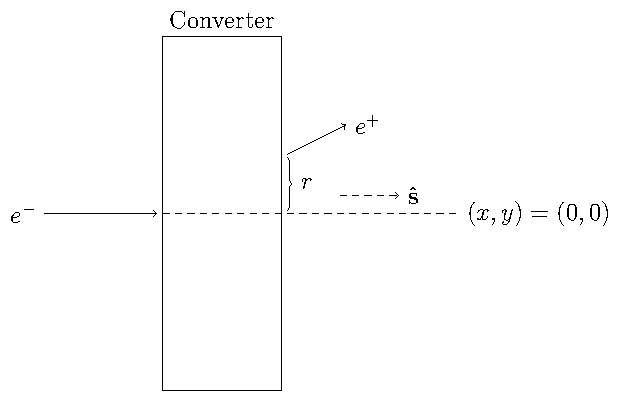
\includegraphics[width=0.6\textwidth]{coords1.pdf}
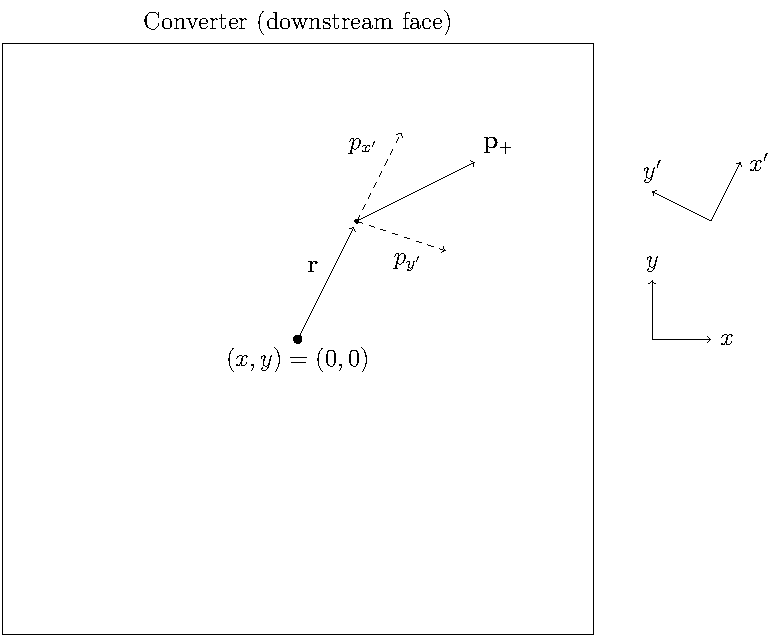
\includegraphics[width=0.8\textwidth]{coords2.pdf}
\caption{Coordinates used to describe the positrons exiting the converter.}
\end{figure}
The incoming electron beam is taken to be along the $z$-axis.
Outgoing positrons will exit the target with some displacement $r$ off of the $z$-axis, and have some energy $E_+$ and momentum $\pp_+$.
It is convenient to define a coordinate system $(x', y', z)$ with $\xx'$ pointing along the direction of $\rr$, and $\yy'$ taken perpendicular to $\xx'$ so that $(x', y', z)$ is a right-handed coordinate system.
This defines $p_x'$ and $p_y'$, the components of the outgoing positron momentum in the primed coordinate system.
We then define the "transverse momenta" $\frac{dx'}{ds}$ and $\frac{dy'}{ds}$ by
\begin{align*}
\frac{dx'}{ds} & = \frac{p_x'}{p_z} \\
\frac{dy'}{ds} & = \frac{p_y'}{p_z}
\end{align*}

\newpage

\section*{The Model}

Given a positron converter of thickness $T$ and incoming electrons of energy $E_-$, we wish to predict $E_+$, $r$, $\frac{dx'}{ds}$, and $\frac{dy'}{ds}$ for the outgoing positrons.
We do this in two steps:
\begin{enumerate}
\item
First, we pull $E_+$ and $r$ from a two-dimensional probability distribution $P(E_+, r)$, which we model as
\begin{align*}
P(E_+, r) & = P_3(E_+) P_3(r) e^{-\alpha E_+} e^{-\beta r} \\
& = C(E_+^3 + A_E E_+^2 + B_E E_+ + C_E) (r^3 + A_r r^2 + B_r r + C_r) e^{-\alpha E_+} e^{-\beta r}
\end{align*}

\item
For outgoing positrons of any given $(E_+, r)$, $\frac{dx'}{ds}$ and $\frac{dy'}{ds}$ are normally distributed.
However, the parameters of these distributions ($\mu$ and $\sigma$) depend on $E_+$ and $r$, with
\begin{align*}
\mu_{dx'/ds}(E_+, r) & = A_x E_+^{\alpha_x} r^{\beta_x} \\
\sigma_{dx'/ds} (E_+, r) & = (a_x + b_x r) (1 - e^{-k_x E_+}) \\
\mu_{dy'/ds} (E_+, r) & = 0 \\
\sigma_{dy'/ds} (E_+, r) & = (a_y + b_y r) (1 - e^{-k_y E_+})
\end{align*}

\end{enumerate}

Note that these functional forms are empirically derived, and are not heavily motivated by the underlying physical processes that occur in the converter.


\section*{Obtaining the Model Coefficients}

Using the Geant4\cite{geant} software package developed at CERN, we have developed a program for simulating the production of positrons in the converter.
Using this program, one can generate data on the number of positrons $N_+$ produced at given $E_+$ and $r$ values, as well as data on $\mu_{dx'/ds}$, $\sigma_{dx'/ds}$, $\mu_{dy'/ds}$, $\sigma_{dy'/ds}$ vs $E_+$ and $r$.
With this data in hand, one can fit the models in the previous section to the data, yielding the fit parameters needed to simulate the converter in \textit{Bmad}.
We have included an \textit{R} script which performs this fitting and outputs the fit parameters.

Note that each of the fit parameters will change for different values of the thickness $T$ and incoming electron energy $E_-$.
As such, it is advised that the simulation and fitting process be performed at several points over the range of $E_-$ and $T$ values of interest.
For each choice of $(E_-, T)$, one set of fit parameters is produced.
\textit{Bmad} then interpolates between the discrete set of $(E_-, T)$ values simulated to model the converter at any electron energy and target thickness in the range of interest.



\printbibliography


\end{document}
